% Options for packages loaded elsewhere
\PassOptionsToPackage{unicode}{hyperref}
\PassOptionsToPackage{hyphens}{url}
%
\documentclass[
]{article}
\usepackage{amsmath,amssymb}
\usepackage{iftex}
\ifPDFTeX
  \usepackage[T1]{fontenc}
  \usepackage[utf8]{inputenc}
  \usepackage{textcomp} % provide euro and other symbols
\else % if luatex or xetex
  \usepackage{unicode-math} % this also loads fontspec
  \defaultfontfeatures{Scale=MatchLowercase}
  \defaultfontfeatures[\rmfamily]{Ligatures=TeX,Scale=1}
\fi
\usepackage{lmodern}
\ifPDFTeX\else
  % xetex/luatex font selection
\fi
% Use upquote if available, for straight quotes in verbatim environments
\IfFileExists{upquote.sty}{\usepackage{upquote}}{}
\IfFileExists{microtype.sty}{% use microtype if available
  \usepackage[]{microtype}
  \UseMicrotypeSet[protrusion]{basicmath} % disable protrusion for tt fonts
}{}
\makeatletter
\@ifundefined{KOMAClassName}{% if non-KOMA class
  \IfFileExists{parskip.sty}{%
    \usepackage{parskip}
  }{% else
    \setlength{\parindent}{0pt}
    \setlength{\parskip}{6pt plus 2pt minus 1pt}}
}{% if KOMA class
  \KOMAoptions{parskip=half}}
\makeatother
\usepackage{xcolor}
\usepackage[margin=1in]{geometry}
\usepackage{color}
\usepackage{fancyvrb}
\newcommand{\VerbBar}{|}
\newcommand{\VERB}{\Verb[commandchars=\\\{\}]}
\DefineVerbatimEnvironment{Highlighting}{Verbatim}{commandchars=\\\{\}}
% Add ',fontsize=\small' for more characters per line
\usepackage{framed}
\definecolor{shadecolor}{RGB}{248,248,248}
\newenvironment{Shaded}{\begin{snugshade}}{\end{snugshade}}
\newcommand{\AlertTok}[1]{\textcolor[rgb]{0.94,0.16,0.16}{#1}}
\newcommand{\AnnotationTok}[1]{\textcolor[rgb]{0.56,0.35,0.01}{\textbf{\textit{#1}}}}
\newcommand{\AttributeTok}[1]{\textcolor[rgb]{0.13,0.29,0.53}{#1}}
\newcommand{\BaseNTok}[1]{\textcolor[rgb]{0.00,0.00,0.81}{#1}}
\newcommand{\BuiltInTok}[1]{#1}
\newcommand{\CharTok}[1]{\textcolor[rgb]{0.31,0.60,0.02}{#1}}
\newcommand{\CommentTok}[1]{\textcolor[rgb]{0.56,0.35,0.01}{\textit{#1}}}
\newcommand{\CommentVarTok}[1]{\textcolor[rgb]{0.56,0.35,0.01}{\textbf{\textit{#1}}}}
\newcommand{\ConstantTok}[1]{\textcolor[rgb]{0.56,0.35,0.01}{#1}}
\newcommand{\ControlFlowTok}[1]{\textcolor[rgb]{0.13,0.29,0.53}{\textbf{#1}}}
\newcommand{\DataTypeTok}[1]{\textcolor[rgb]{0.13,0.29,0.53}{#1}}
\newcommand{\DecValTok}[1]{\textcolor[rgb]{0.00,0.00,0.81}{#1}}
\newcommand{\DocumentationTok}[1]{\textcolor[rgb]{0.56,0.35,0.01}{\textbf{\textit{#1}}}}
\newcommand{\ErrorTok}[1]{\textcolor[rgb]{0.64,0.00,0.00}{\textbf{#1}}}
\newcommand{\ExtensionTok}[1]{#1}
\newcommand{\FloatTok}[1]{\textcolor[rgb]{0.00,0.00,0.81}{#1}}
\newcommand{\FunctionTok}[1]{\textcolor[rgb]{0.13,0.29,0.53}{\textbf{#1}}}
\newcommand{\ImportTok}[1]{#1}
\newcommand{\InformationTok}[1]{\textcolor[rgb]{0.56,0.35,0.01}{\textbf{\textit{#1}}}}
\newcommand{\KeywordTok}[1]{\textcolor[rgb]{0.13,0.29,0.53}{\textbf{#1}}}
\newcommand{\NormalTok}[1]{#1}
\newcommand{\OperatorTok}[1]{\textcolor[rgb]{0.81,0.36,0.00}{\textbf{#1}}}
\newcommand{\OtherTok}[1]{\textcolor[rgb]{0.56,0.35,0.01}{#1}}
\newcommand{\PreprocessorTok}[1]{\textcolor[rgb]{0.56,0.35,0.01}{\textit{#1}}}
\newcommand{\RegionMarkerTok}[1]{#1}
\newcommand{\SpecialCharTok}[1]{\textcolor[rgb]{0.81,0.36,0.00}{\textbf{#1}}}
\newcommand{\SpecialStringTok}[1]{\textcolor[rgb]{0.31,0.60,0.02}{#1}}
\newcommand{\StringTok}[1]{\textcolor[rgb]{0.31,0.60,0.02}{#1}}
\newcommand{\VariableTok}[1]{\textcolor[rgb]{0.00,0.00,0.00}{#1}}
\newcommand{\VerbatimStringTok}[1]{\textcolor[rgb]{0.31,0.60,0.02}{#1}}
\newcommand{\WarningTok}[1]{\textcolor[rgb]{0.56,0.35,0.01}{\textbf{\textit{#1}}}}
\usepackage{graphicx}
\makeatletter
\def\maxwidth{\ifdim\Gin@nat@width>\linewidth\linewidth\else\Gin@nat@width\fi}
\def\maxheight{\ifdim\Gin@nat@height>\textheight\textheight\else\Gin@nat@height\fi}
\makeatother
% Scale images if necessary, so that they will not overflow the page
% margins by default, and it is still possible to overwrite the defaults
% using explicit options in \includegraphics[width, height, ...]{}
\setkeys{Gin}{width=\maxwidth,height=\maxheight,keepaspectratio}
% Set default figure placement to htbp
\makeatletter
\def\fps@figure{htbp}
\makeatother
\setlength{\emergencystretch}{3em} % prevent overfull lines
\providecommand{\tightlist}{%
  \setlength{\itemsep}{0pt}\setlength{\parskip}{0pt}}
\setcounter{secnumdepth}{-\maxdimen} % remove section numbering
\ifLuaTeX
  \usepackage{selnolig}  % disable illegal ligatures
\fi
\IfFileExists{bookmark.sty}{\usepackage{bookmark}}{\usepackage{hyperref}}
\IfFileExists{xurl.sty}{\usepackage{xurl}}{} % add URL line breaks if available
\urlstyle{same}
\hypersetup{
  pdftitle={VoI book code: Case study and guidelines for estimating EVPPI using regression in R},
  hidelinks,
  pdfcreator={LaTeX via pandoc}}

\title{VoI book code: Case study and guidelines for estimating EVPPI
using regression in R}
\author{}
\date{\vspace{-2.5em}}

\begin{document}
\maketitle

Change this path to reflect where you downloaded the Chemotherapy\_Book
repository.

This block of code is only needed if you want to compile this
\texttt{Rmd} source file into a document.

Draw a sample from probabilistic analysis of the model.

\begin{Shaded}
\begin{Highlighting}[]
\FunctionTok{source}\NormalTok{(}\StringTok{"04\_analysis/01\_model\_run.R"}\NormalTok{)}
\NormalTok{nb }\OtherTok{\textless{}{-}}\NormalTok{ m\_net\_benefit[ , , wtp\_seq }\SpecialCharTok{==} \DecValTok{20000}\NormalTok{]}
\end{Highlighting}
\end{Shaded}

\hypertarget{calculating-single-parameter-evppi.}{%
\subsection{Calculating single-parameter
EVPPI.}\label{calculating-single-parameter-evppi.}}

Calculate the single-parameter EVPPI for all the parameters in the
model. This returns a data frame containing the EVPPI estimates.

\begin{Shaded}
\begin{Highlighting}[]
\FunctionTok{library}\NormalTok{(voi)}
\NormalTok{pars\_all }\OtherTok{\textless{}{-}} \FunctionTok{as.list}\NormalTok{(}\FunctionTok{names}\NormalTok{(m\_params))}
\NormalTok{ev\_single }\OtherTok{\textless{}{-}} \FunctionTok{evppi}\NormalTok{(}\AttributeTok{outputs=}\NormalTok{nb, }\AttributeTok{inputs=}\NormalTok{m\_params, }\AttributeTok{pars=}\NormalTok{pars\_all)}
\NormalTok{ev\_single}
\end{Highlighting}
\end{Shaded}

\begin{verbatim}
##                    pars    evppi
## 1     p_side_effects_t1  24.7915
## 2     p_side_effects_t2 260.9055
## 3           c_home_care   0.0000
## 4            c_hospital   0.0032
## 5               c_death   0.0000
## 6            u_recovery   7.7910
## 7           u_home_care 103.7762
## 8            u_hospital   2.6355
## 9    logor_side_effects 329.0098
## 10 p_hospitalised_total  21.8343
## 11               p_died  41.5116
## 12          lambda_home  10.0146
## 13          lambda_hosp  21.7919
## 14        rate_longterm  38.9335
\end{verbatim}

Dot-plot of the estimates, sorted with the highest values at the top.

\begin{Shaded}
\begin{Highlighting}[]
\FunctionTok{plot}\NormalTok{(ev\_single, }\AttributeTok{order =} \ConstantTok{TRUE}\NormalTok{)}
\end{Highlighting}
\end{Shaded}

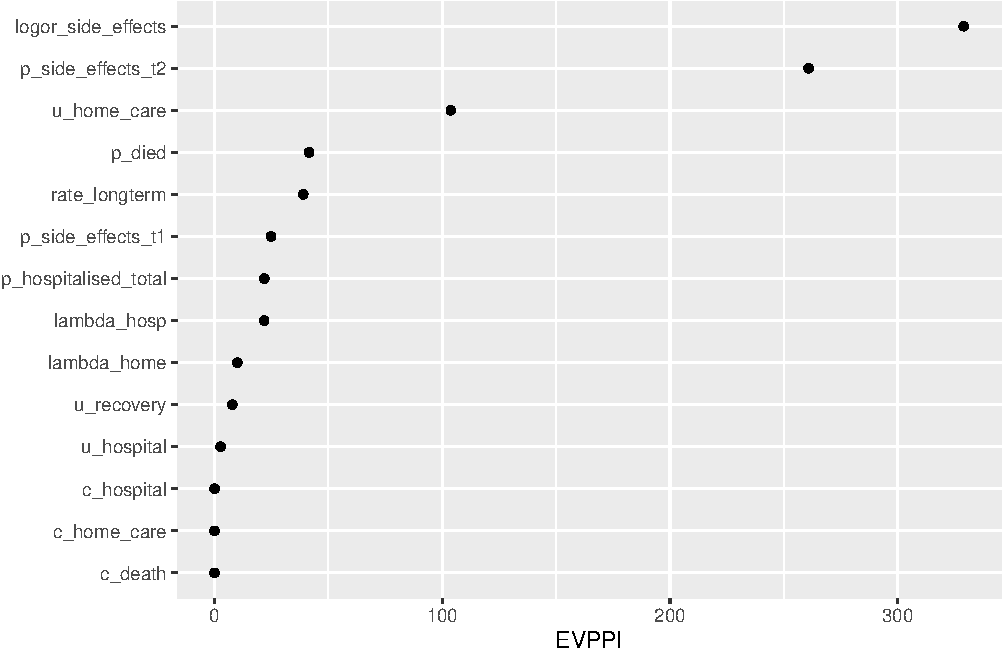
\includegraphics{evppi_reg_files/figure-latex/dotplot-1.pdf}

Single-parameter EVPPIs for a specified subset of parameters.

\begin{Shaded}
\begin{Highlighting}[]
\FunctionTok{evppi}\NormalTok{(}\AttributeTok{outputs=}\NormalTok{nb, }\AttributeTok{inputs=}\NormalTok{m\_params, }
      \AttributeTok{pars=}\FunctionTok{list}\NormalTok{(}\StringTok{"logor\_side\_effects"}\NormalTok{, }\StringTok{"p\_side\_effects\_t1"}\NormalTok{, }\StringTok{"u\_hospital"}\NormalTok{))}
\end{Highlighting}
\end{Shaded}

Multi-parameter EVPPI for four groups of parameters: those associated
with side effects, transition probabilites, costs and utilities
respectively.

\begin{Shaded}
\begin{Highlighting}[]
\NormalTok{par\_groups }\OtherTok{\textless{}{-}} \FunctionTok{list}\NormalTok{(}
  \StringTok{"side\_effects"} \OtherTok{=} \FunctionTok{c}\NormalTok{(}\StringTok{"p\_side\_effects\_t1"}\NormalTok{,}\StringTok{"logor\_side\_effects"}\NormalTok{),}
  \StringTok{"trans\_probs"} \OtherTok{=} \FunctionTok{c}\NormalTok{(}\StringTok{"p\_hospitalised\_total"}\NormalTok{,}\StringTok{"p\_died"}\NormalTok{,}
                    \StringTok{"lambda\_home"}\NormalTok{,}\StringTok{"lambda\_hosp"}\NormalTok{),}
  \StringTok{"costs"} \OtherTok{=} \FunctionTok{c}\NormalTok{(}\StringTok{"c\_home\_care"}\NormalTok{,}\StringTok{"c\_hospital"}\NormalTok{,}\StringTok{"c\_death"}\NormalTok{),}
  \StringTok{"utilities"} \OtherTok{=} \FunctionTok{c}\NormalTok{(}\StringTok{"u\_recovery"}\NormalTok{,}\StringTok{"u\_home\_care"}\NormalTok{,}\StringTok{"u\_hospital"}\NormalTok{)}
\NormalTok{)}
\NormalTok{ev\_grouped }\OtherTok{\textless{}{-}} \FunctionTok{evppi}\NormalTok{(}\AttributeTok{outputs=}\NormalTok{nb, }\AttributeTok{inputs=}\NormalTok{m\_params, }\AttributeTok{pars=}\NormalTok{par\_groups)}
\NormalTok{ev\_grouped}
\end{Highlighting}
\end{Shaded}

\begin{verbatim}
##           pars  evppi
## 1 side_effects 330.62
## 2  trans_probs  63.14
## 3        costs   7.01
## 4    utilities 105.22
\end{verbatim}

In this example, it is clear that the parameters associated with the
risk of side effects have the greatest EVPPI.

\hypertarget{checking-regression-models-for-evppi-calculation}{%
\subsection{Checking regression models for EVPPI
calculation}\label{checking-regression-models-for-evppi-calculation}}

Figure shown in the book

\begin{Shaded}
\begin{Highlighting}[]
\NormalTok{ev\_single }\OtherTok{\textless{}{-}} \FunctionTok{evppi}\NormalTok{(}\AttributeTok{outputs=}\NormalTok{nb, }\AttributeTok{inputs=}\NormalTok{m\_params, }\AttributeTok{pars=}\NormalTok{pars\_all, }\AttributeTok{check=}\ConstantTok{TRUE}\NormalTok{)}
\FunctionTok{check\_regression}\NormalTok{(ev\_single, }\AttributeTok{pars =} \StringTok{"logor\_side\_effects"}\NormalTok{)}
\end{Highlighting}
\end{Shaded}

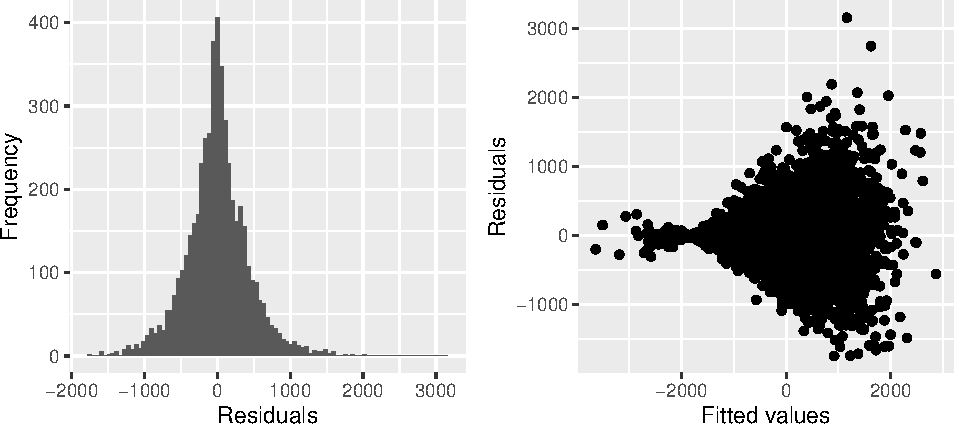
\includegraphics{evppi_reg_files/figure-latex/regression_diagnostics-1.pdf}

Additional analysis with standard errors:

\begin{Shaded}
\begin{Highlighting}[]
\FunctionTok{evppi}\NormalTok{(}\AttributeTok{outputs=}\NormalTok{nb, }\AttributeTok{inputs=}\NormalTok{m\_params,}
      \AttributeTok{pars =} \FunctionTok{list}\NormalTok{(}\StringTok{"p\_side\_effects\_t2"}\NormalTok{,}\StringTok{"u\_hospital"}\NormalTok{), }\AttributeTok{se=}\ConstantTok{TRUE}\NormalTok{)}
\end{Highlighting}
\end{Shaded}

Alternative regression models:

\begin{Shaded}
\begin{Highlighting}[]
\FunctionTok{evppi}\NormalTok{(}\AttributeTok{outputs=}\NormalTok{nb, }\AttributeTok{inputs=}\NormalTok{m\_params,}
      \AttributeTok{pars =} \FunctionTok{list}\NormalTok{(}\StringTok{"p\_side\_effects\_t2"}\NormalTok{,}\StringTok{"u\_hospital"}\NormalTok{))}
\end{Highlighting}
\end{Shaded}

\begin{verbatim}
##                pars  evppi
## 1 p_side_effects_t2 260.91
## 2        u_hospital   2.64
\end{verbatim}

\begin{Shaded}
\begin{Highlighting}[]
\FunctionTok{evppi}\NormalTok{(}\AttributeTok{outputs=}\NormalTok{nb, }\AttributeTok{inputs=}\NormalTok{m\_params,}
      \AttributeTok{pars =} \FunctionTok{list}\NormalTok{(}\StringTok{"p\_side\_effects\_t2"}\NormalTok{,}\StringTok{"u\_hospital"}\NormalTok{),}
      \AttributeTok{method=}\StringTok{"earth"}\NormalTok{)}
\end{Highlighting}
\end{Shaded}

\begin{verbatim}
##                pars evppi
## 1 p_side_effects_t2   262
## 2        u_hospital     0
\end{verbatim}

\hypertarget{comparing-different-regression-specifications-single-parameter-evppi}{%
\subsection{Comparing different regression specifications:
single-parameter
EVPPI}\label{comparing-different-regression-specifications-single-parameter-evppi}}

\begin{Shaded}
\begin{Highlighting}[]
\NormalTok{(e1 }\OtherTok{\textless{}{-}} \FunctionTok{evppi}\NormalTok{(}\AttributeTok{outputs=}\NormalTok{nb, }\AttributeTok{inputs=}\NormalTok{m\_params, }\AttributeTok{pars=}\NormalTok{par\_groups[}\DecValTok{1}\NormalTok{], }\AttributeTok{check=}\ConstantTok{TRUE}\NormalTok{))}
\end{Highlighting}
\end{Shaded}

\begin{verbatim}
##           pars evppi
## 1 side_effects   331
\end{verbatim}

\begin{Shaded}
\begin{Highlighting}[]
\NormalTok{(e2 }\OtherTok{\textless{}{-}} \FunctionTok{evppi}\NormalTok{(}\AttributeTok{outputs=}\NormalTok{nb, }\AttributeTok{inputs=}\NormalTok{m\_params, }\AttributeTok{pars=}\NormalTok{par\_groups[}\DecValTok{1}\NormalTok{], }
             \AttributeTok{gam\_formula=}\StringTok{"s(p\_side\_effects\_t1) + s(logor\_side\_effects)"}\NormalTok{, }\AttributeTok{check=}\ConstantTok{TRUE}\NormalTok{))}
\end{Highlighting}
\end{Shaded}

\begin{verbatim}
##           pars evppi
## 1 side_effects   332
\end{verbatim}

\begin{Shaded}
\begin{Highlighting}[]
\FunctionTok{check\_regression}\NormalTok{(e1, }\AttributeTok{plot=}\ConstantTok{FALSE}\NormalTok{)}
\end{Highlighting}
\end{Shaded}

\begin{verbatim}
## $AIC
## [1] 74754
\end{verbatim}

\begin{Shaded}
\begin{Highlighting}[]
\FunctionTok{check\_regression}\NormalTok{(e2, }\AttributeTok{plot=}\ConstantTok{FALSE}\NormalTok{)}
\end{Highlighting}
\end{Shaded}

\begin{verbatim}
## $AIC
## [1] 74838
\end{verbatim}

\texttt{earth} models with two-way versus three-way interactions

\begin{Shaded}
\begin{Highlighting}[]
\NormalTok{(e1 }\OtherTok{\textless{}{-}} \FunctionTok{evppi}\NormalTok{(}\AttributeTok{outputs=}\NormalTok{nb, }\AttributeTok{inputs=}\NormalTok{m\_params, }\AttributeTok{pars=}\NormalTok{par\_groups[}\DecValTok{1}\NormalTok{], }\AttributeTok{method =} \StringTok{"earth"}\NormalTok{, }\AttributeTok{check=}\ConstantTok{TRUE}\NormalTok{))}
\end{Highlighting}
\end{Shaded}

\begin{verbatim}
##           pars evppi
## 1 side_effects   334
\end{verbatim}

\begin{Shaded}
\begin{Highlighting}[]
\NormalTok{(e2 }\OtherTok{\textless{}{-}} \FunctionTok{evppi}\NormalTok{(}\AttributeTok{outputs=}\NormalTok{nb, }\AttributeTok{inputs=}\NormalTok{m\_params, }\AttributeTok{pars=}\NormalTok{par\_groups[}\DecValTok{1}\NormalTok{], }\AttributeTok{method =} \StringTok{"earth"}\NormalTok{, }
             \AttributeTok{degree=}\DecValTok{3}\NormalTok{, }\AttributeTok{check=}\ConstantTok{TRUE}\NormalTok{))}
\end{Highlighting}
\end{Shaded}

\begin{verbatim}
##           pars evppi
## 1 side_effects   333
\end{verbatim}

\begin{Shaded}
\begin{Highlighting}[]
\FunctionTok{check\_regression}\NormalTok{(e1,}\AttributeTok{plot=}\ConstantTok{FALSE}\NormalTok{)}
\end{Highlighting}
\end{Shaded}

\begin{verbatim}
## $gcv
## [1] 185678
\end{verbatim}

\begin{Shaded}
\begin{Highlighting}[]
\FunctionTok{check\_regression}\NormalTok{(e2,}\AttributeTok{plot=}\ConstantTok{FALSE}\NormalTok{)}
\end{Highlighting}
\end{Shaded}

\begin{verbatim}
## $gcv
## [1] 183384
\end{verbatim}

\hypertarget{comparing-different-regression-specifications-multi-parameter-evppi}{%
\subsection{Comparing different regression specifications:
multi-parameter
EVPPI}\label{comparing-different-regression-specifications-multi-parameter-evppi}}

\begin{Shaded}
\begin{Highlighting}[]
\NormalTok{costs\_utilities }\OtherTok{\textless{}{-}} \FunctionTok{c}\NormalTok{(par\_groups}\SpecialCharTok{$}\NormalTok{costs, par\_groups}\SpecialCharTok{$}\NormalTok{utilities)}
\NormalTok{ev1 }\OtherTok{\textless{}{-}} \FunctionTok{evppi}\NormalTok{(}\AttributeTok{outputs=}\NormalTok{nb, }\AttributeTok{inputs=}\NormalTok{m\_params, }\AttributeTok{pars=}\NormalTok{costs\_utilities, }\AttributeTok{method=}\StringTok{"gam"}\NormalTok{, }
             \AttributeTok{gam\_formula =} \StringTok{"s(c\_home\_care) + s(c\_hospital) + s(c\_death) + }
\StringTok{                            s(u\_recovery) + s(u\_home\_care) + s(u\_hospital)"}\NormalTok{,}
             \AttributeTok{check=}\ConstantTok{TRUE}\NormalTok{)}
\NormalTok{ev2 }\OtherTok{\textless{}{-}} \FunctionTok{evppi}\NormalTok{(}\AttributeTok{outputs=}\NormalTok{nb, }\AttributeTok{inputs=}\NormalTok{m\_params, }\AttributeTok{pars=}\NormalTok{costs\_utilities, }\AttributeTok{method=}\StringTok{"gam"}\NormalTok{, }
             \AttributeTok{gam\_formula =} \FunctionTok{all\_interactions}\NormalTok{(costs\_utilities, }\DecValTok{2}\NormalTok{), }\AttributeTok{check=}\ConstantTok{TRUE}\NormalTok{) }
\NormalTok{ev3 }\OtherTok{\textless{}{-}} \FunctionTok{evppi}\NormalTok{(}\AttributeTok{outputs=}\NormalTok{nb, }\AttributeTok{inputs=}\NormalTok{m\_params, }\AttributeTok{pars=}\NormalTok{costs\_utilities, }\AttributeTok{method=}\StringTok{"earth"}\NormalTok{, }\AttributeTok{check=}\ConstantTok{TRUE}\NormalTok{)}
\NormalTok{ev4 }\OtherTok{\textless{}{-}} \FunctionTok{evppi}\NormalTok{(}\AttributeTok{outputs=}\NormalTok{nb, }\AttributeTok{inputs=}\NormalTok{m\_params, }\AttributeTok{pars=}\NormalTok{costs\_utilities, }\AttributeTok{method=}\StringTok{"earth"}\NormalTok{, }
             \AttributeTok{degree=}\DecValTok{2}\NormalTok{, }\AttributeTok{check=}\ConstantTok{TRUE}\NormalTok{)}
\NormalTok{ev5 }\OtherTok{\textless{}{-}} \FunctionTok{evppi}\NormalTok{(}\AttributeTok{outputs=}\NormalTok{nb, }\AttributeTok{inputs=}\NormalTok{m\_params, }\AttributeTok{pars=}\NormalTok{costs\_utilities, }\AttributeTok{method=}\StringTok{"gp"}\NormalTok{) }
\NormalTok{ev6 }\OtherTok{\textless{}{-}} \FunctionTok{evppi}\NormalTok{(}\AttributeTok{outputs=}\NormalTok{nb, }\AttributeTok{inputs=}\NormalTok{m\_params, }\AttributeTok{pars=}\NormalTok{costs\_utilities, }\AttributeTok{method=}\StringTok{"inla"}\NormalTok{) }
\end{Highlighting}
\end{Shaded}


\end{document}
